\chapter{Result}


\begin{figure}[h]
 \begin{center}
  \includegraphics[width=1.0\textwidth]{simulation.eps}
 \end{center}
 \caption{A view of our flock simulation system. The ball on the left is the target for navigating flocks.}
 \label{figure:simulation}
\end{figure}


\section{Flock simulation for generating input video}


For testing our method, a video with bird flock is needed. We planned to use real bird video at first. However, after searching for real bird videos, we found that videos we can find are not good enough as input video, since our approach has several assumptions: all birds stay in the view of camera, and camera is not moving. We also captured various bird videos, but it is still difficult to obtain enough videos that satisfy the assumptions.


Due to difficulties mentioned above, other than using real bird video, we further implemented a bird flock simulation system and capture the flock motion as input video to test our method. The simulation system is based on boid model, which assumes a flock is simply the result of the interaction between the behaviors of individual birds. With these behaviors, the system can produce fine flock motion with numbers of birds. However, boid model can only model flock wandering behavior. That is, after assigning initial parameters, all birds become uncontrollable during the simulation, and the simulation always produces same results. To keep the diversity of the generated simulation result, we further include the homing behavior introduced in \cite{Shape,OB1}. With this behavior, we can generate different flock motions efficiently with various different results. After the simulation result is generated, we capture videos from a view. The captured video is then used as an input video to the system. Figure \ref{figure:simulation} shows a view of our flock simulation system.


\section{Generated flock motion}


We have tested our with various bird videos. Here we show three representative results. The first one is a real bird video taken with RGB camera by ourselves, while the other two are generated input videos from our flock simulation system.  Information and parameters of three input videos are shown in Table \ref{table:result}.


\begin{table}[h]
\begin{tabular}{|l|l|l|l|l|l|l|l|l|}
\hline
  & resolution & bird num & frame num & $v_{target}$ & $\lambda_{t}$ & $\lambda_{f}$ & $w_{sep}$ & $d_{sep}$ \\ \hline
Result 1& 854x480    & 4           & 120          & 0.1          & 0.3           & 1.0           & 2         & 0.9       \\ \hline
Result 2& 1280x720   & 10          & 340          & 0.1          & 0.3           & 1.0          & 2         & 0.9         \\ \hline
Result 3& 1280x720   & 5           & 230          & 0.5          & 0.3           & 0.1           & 2         & 0.8       \\ \hline
\end{tabular}
\caption{Information and optimization parameters of 3 input videos.}
\label{table:result}
\end{table}


%\begin{figure}[h]
% \begin{center}
%  \includegraphics[width=1.0\textwidth]{result1.eps}
% \end{center}
% \caption{Result1:(top)input video. (middle)generated result from side view. (bottom)generated result from top view.}
% \label{figure:result1_side}
%\end{figure}


Figure \ref{figure:result1_com} shows our first result generated with real bird video as input. The input video is relatively short and has 4 birds. Camera also slightly moves during recording. Although the quality of the input video is not good, we test our system with this real video before using generated videos as input to claim that our system can be used on real bird videos. Results of 3 frames in time sequence are shown in Figure \ref{figure:result1_com}. The first row is the input video, and the second, third rows are generated flock motions from our system, in camera view and top view.



\begin{figure}[h]
\begin{center}
\subfloat[Input video]{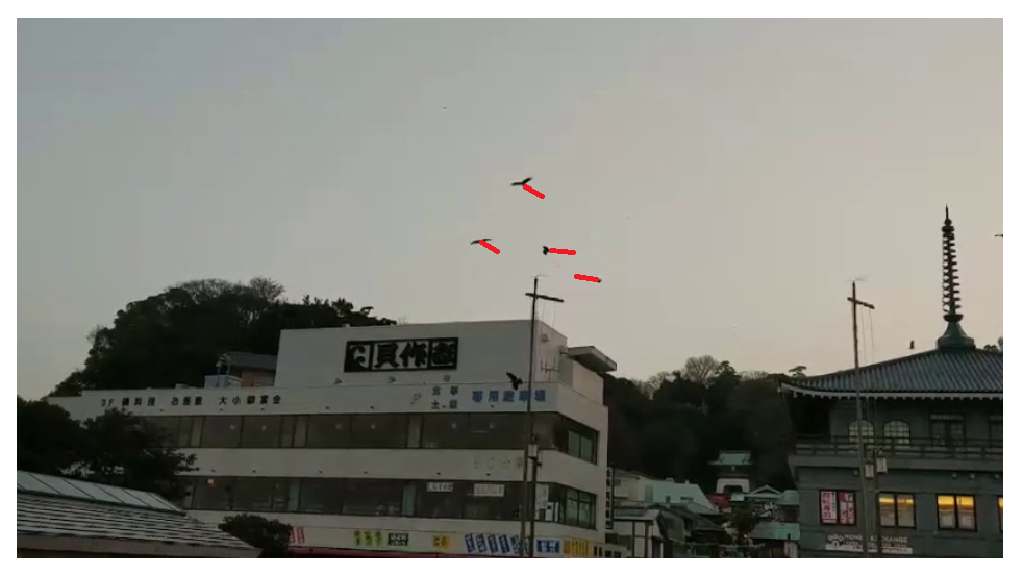
\includegraphics[width=.3\textwidth]{result_1_input_40.eps}}\hspace{\fill}
\subfloat[]{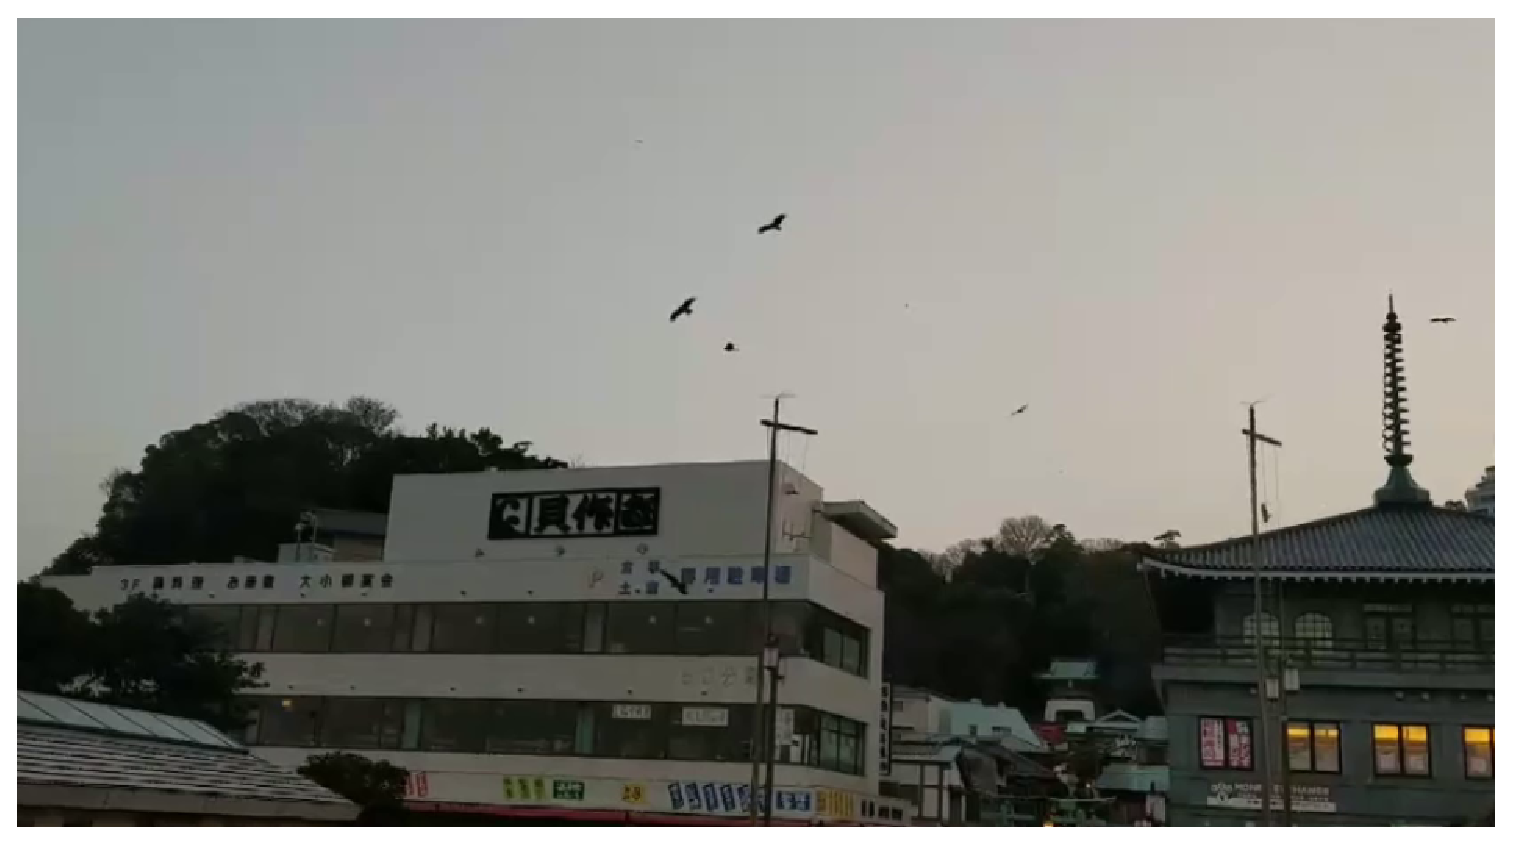
\includegraphics[width=.3\textwidth]{result_1_input_60.eps}}\hspace{\fill}
\subfloat[]{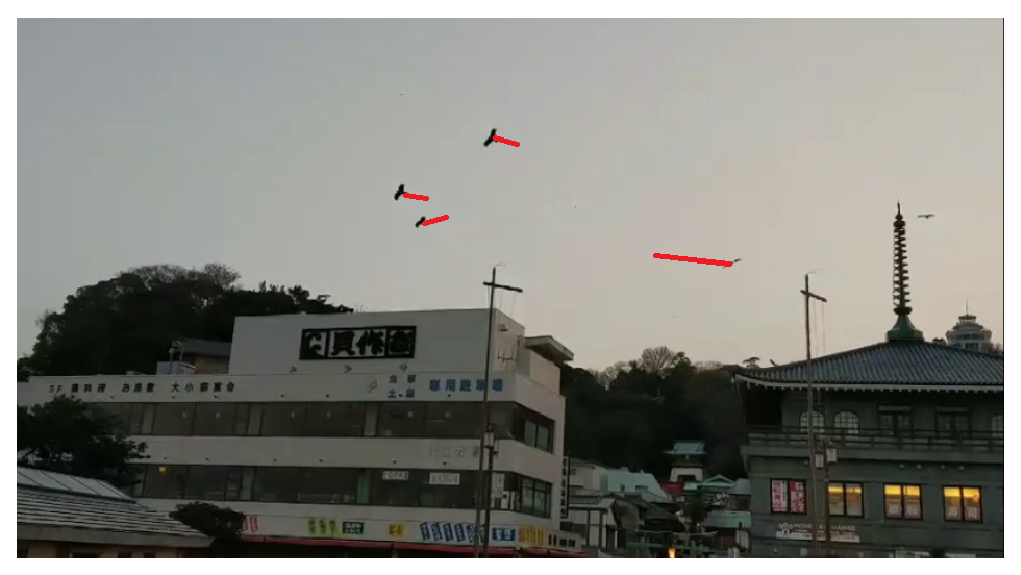
\includegraphics[width=.3\textwidth]{result_1_input_80.eps}}


\subfloat[Result (camera view)]{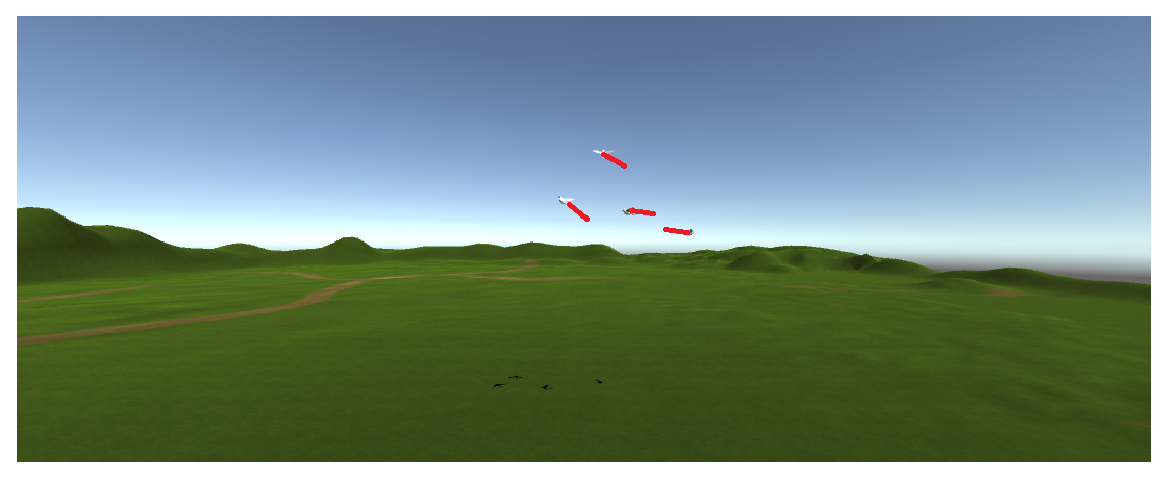
\includegraphics[width=.3\textwidth]{result_1_side_40.eps}}\hspace{\fill}
\subfloat[]{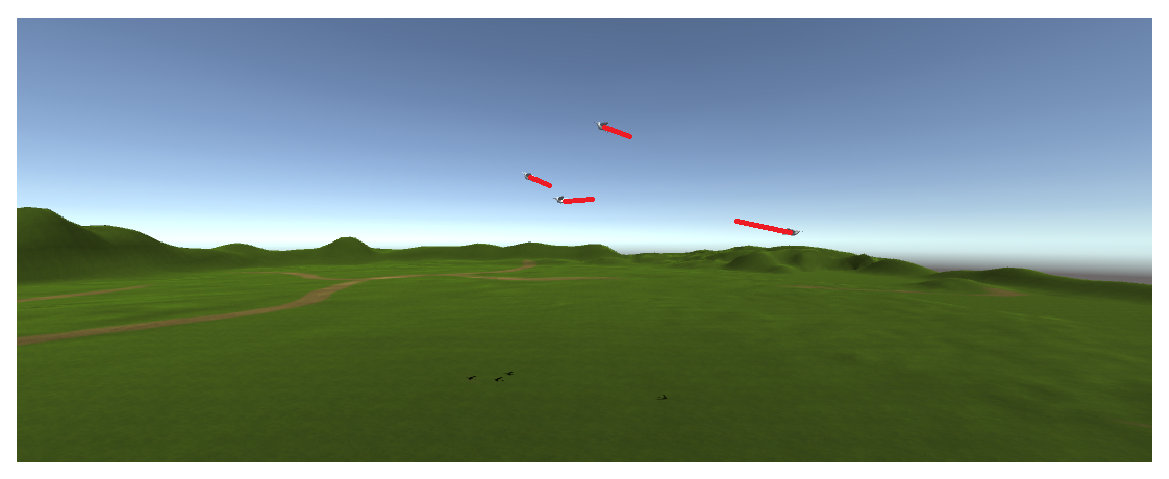
\includegraphics[width=.3\textwidth]{result_1_side_60.eps}}\hspace{\fill}
\subfloat[]{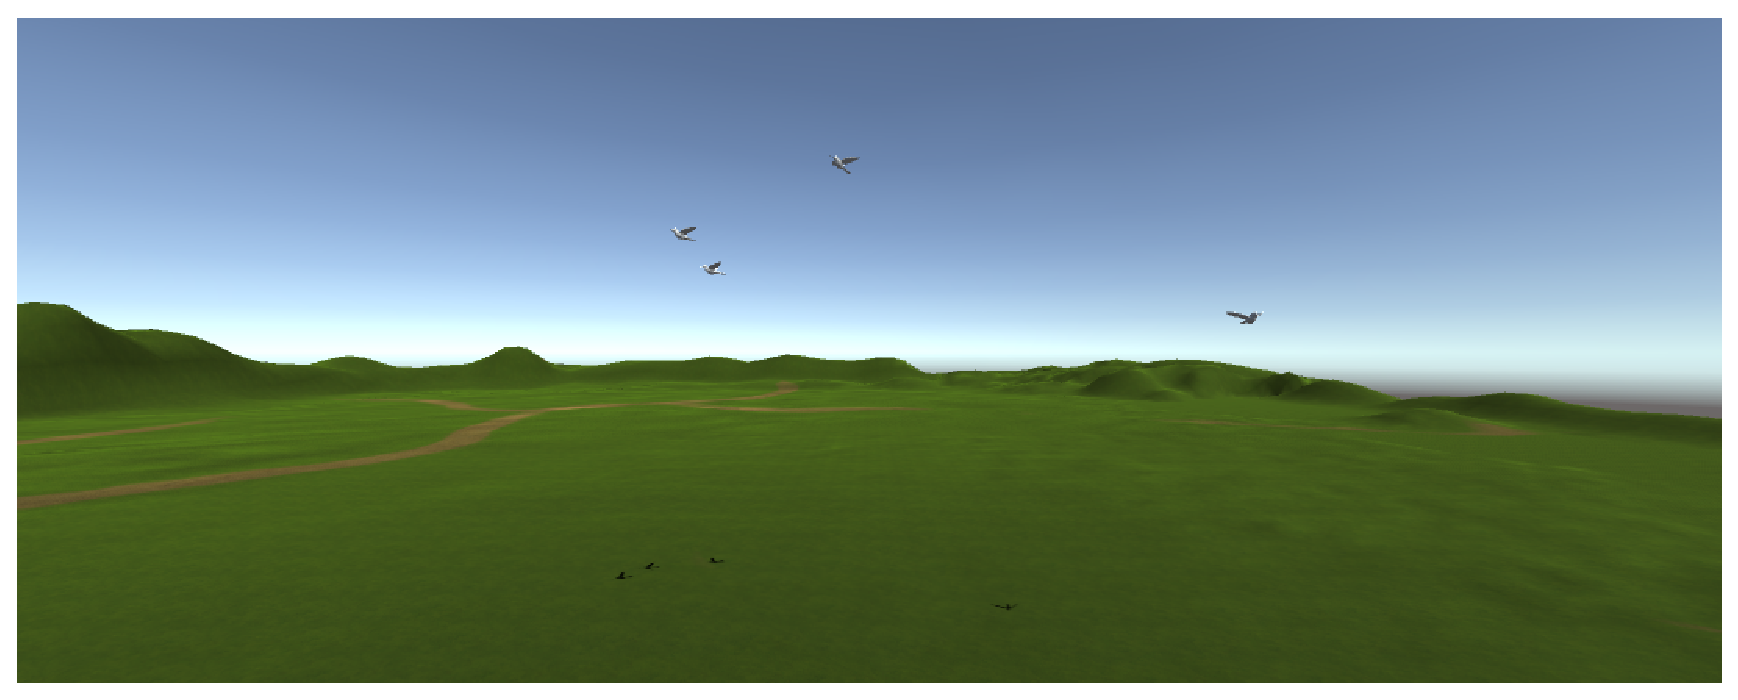
\includegraphics[width=.3\textwidth]{result_1_side_80.eps}}


\subfloat[Result (top view)]{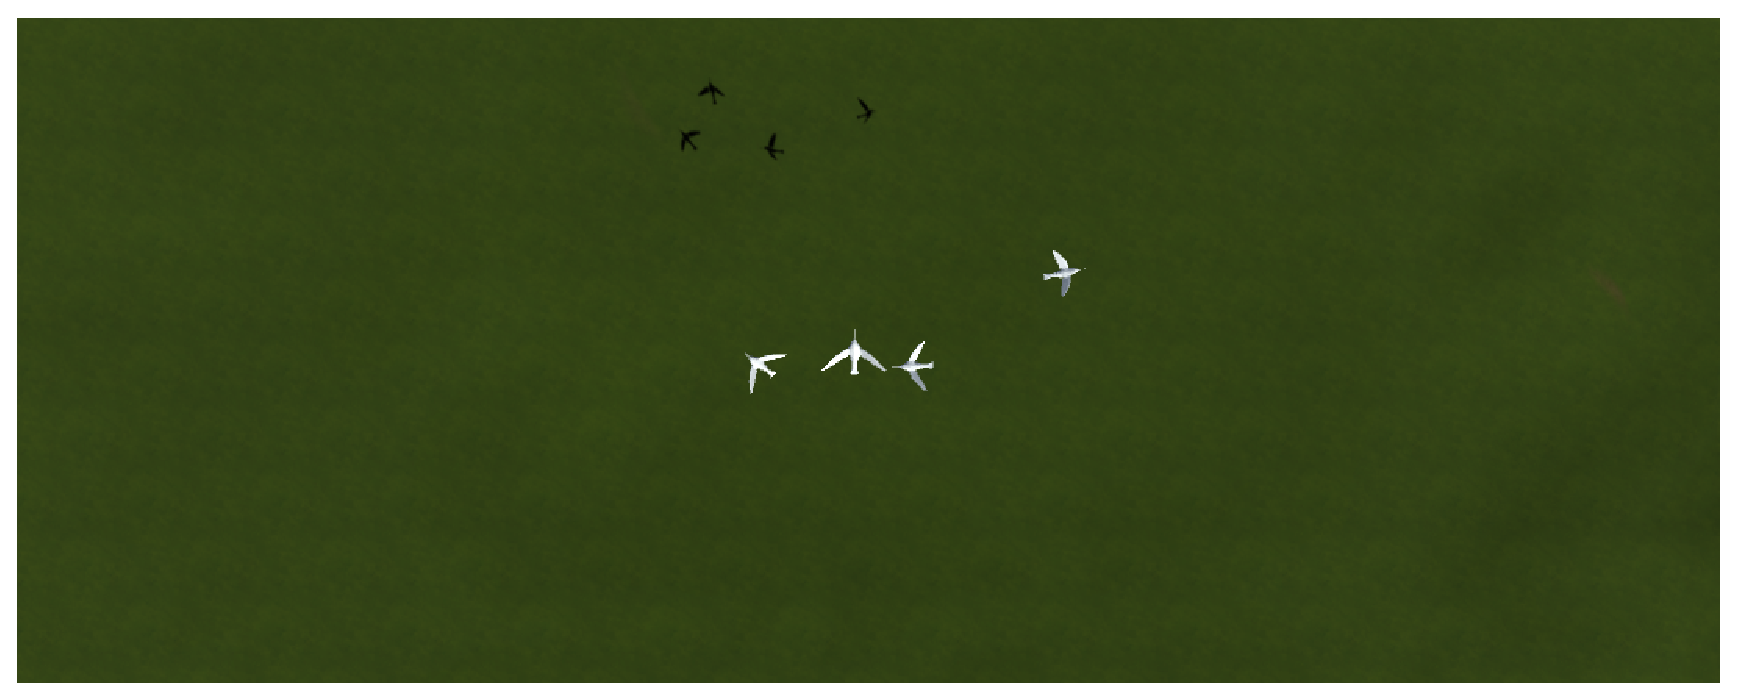
\includegraphics[width=.3\textwidth]{result_1_top_40.eps}}\hspace{\fill}
\subfloat[]{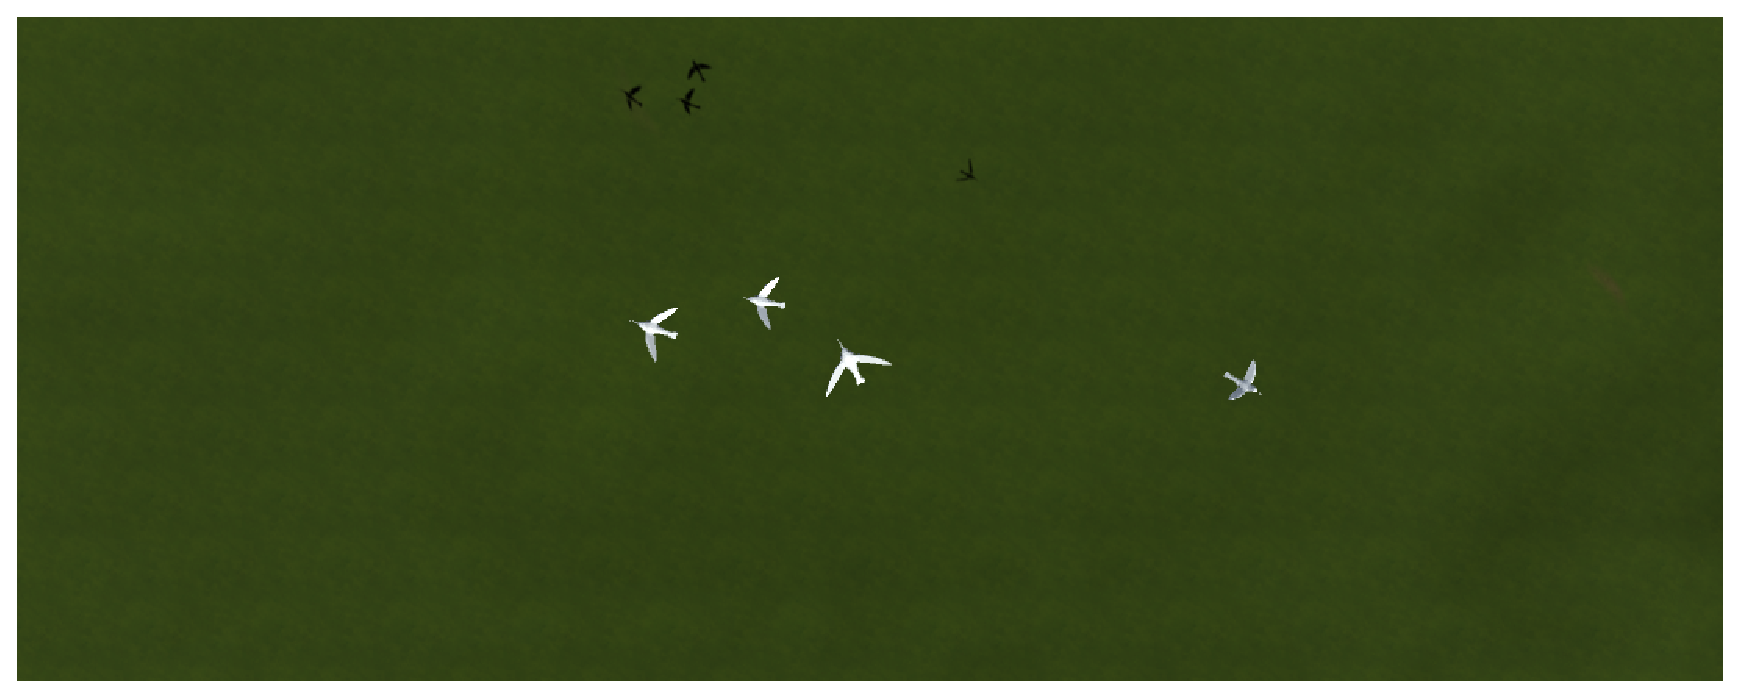
\includegraphics[width=.3\textwidth]{result_1_top_60.eps}}\hspace{\fill}
\subfloat[]{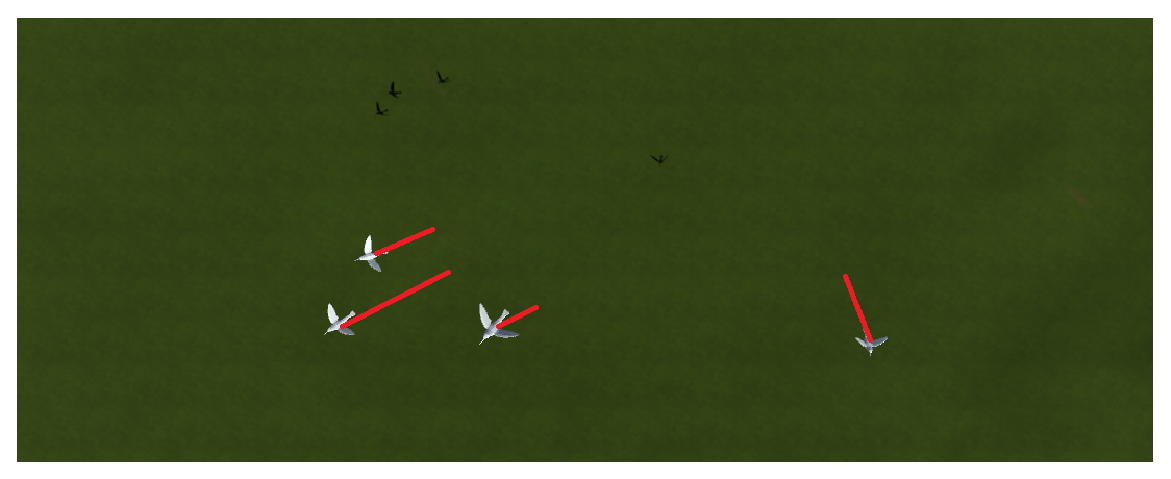
\includegraphics[width=.3\textwidth]{result_1_top_80.eps}}
\end{center}
\caption{Comparison of Result 1 in frame 40, 60, 80. Red lines are bird trajectories in previous frames. }
\label{figure:result1_com}
\end{figure}


By comparing between the input video (a) (b) (c) and generated result in camera view (d)(e)(f), it can be observed that the trajectories of all birds are exactly same, since two-dimensional projection is used as a constraint in the optimization stage. This shows that our optimization algorithm retain the track information from the original video. To confirm whether the depth is properly predicted, we check the result motion from another view from top, shown in (g)(h)(i). Since this result contains only four birds, it is more difficult to observe flock behavior. However, by in (g) and (h), we can still observe that two birds avoid each other when they are two close, showing that flock behavior has its functionality.


An experiment has also be done with this video input to further examine the functionality of the flock behavior similarity term in our error function. We generated two different result, with one applying flock behavior similarity term, and one disabling the term by setting $\lambda_{f}$ to 0. Figure \ref{figure:collide} shows the result. Figure \ref{figure:collide} shows the particular frame when colliding happens. In (a) and (b), representing results in camera view, we can observe that two birds overlap with each other in camera view. In another view (c) and (d), we can see that, with the flock similarity term being active, the two birds does not collide in (c), while birds collide in (d). This shows that the functionality of flock behavior similarity term works well, since it is defined to keep birds in flock from colliding with each others while keeping the flock together.


\begin{figure}[h]
\begin{center}
\subfloat[Result with $\lambda_{f}=1.0$ (camera view)]{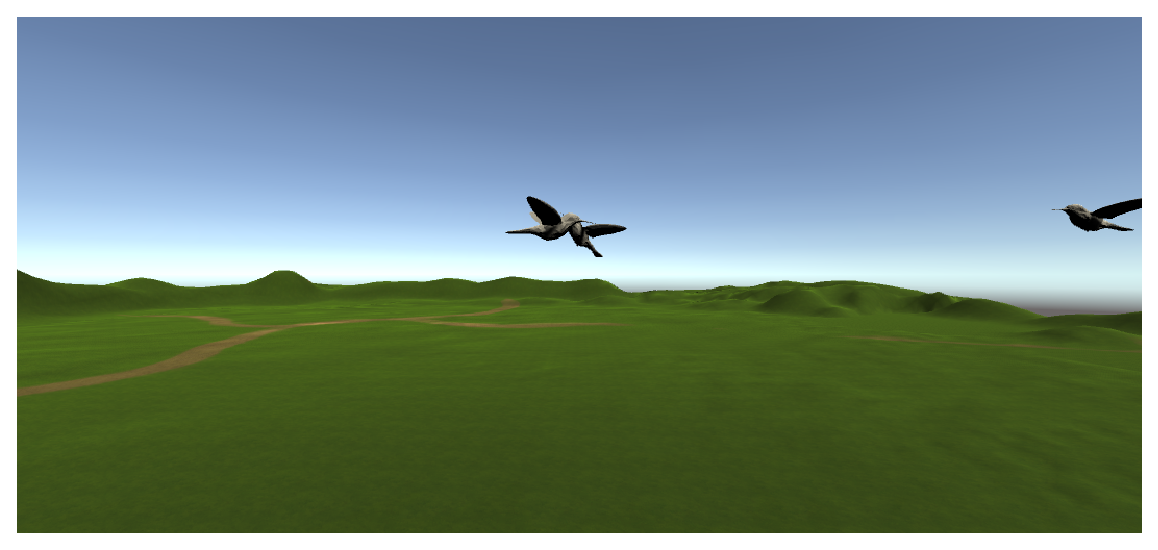
\includegraphics[width=.4\textwidth]{avoid_side.eps}}\hspace{\fill}
\subfloat[Result with $\lambda_{f}=0$ (camera view)]{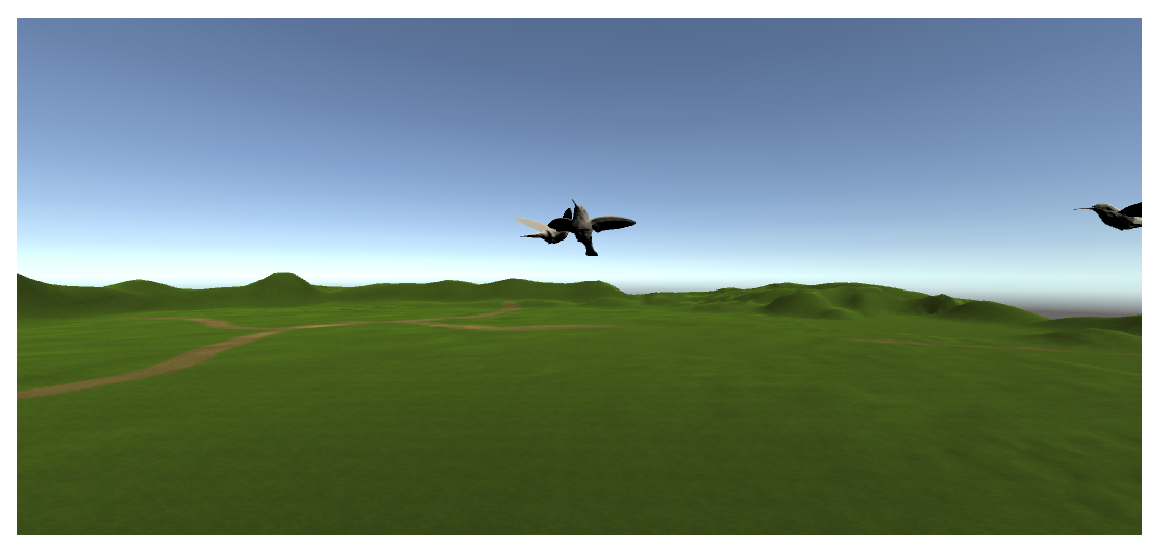
\includegraphics[width=.4\textwidth]{collide_side.eps}}


\subfloat[Result with $\lambda_{f}=1.0$ (top view)]{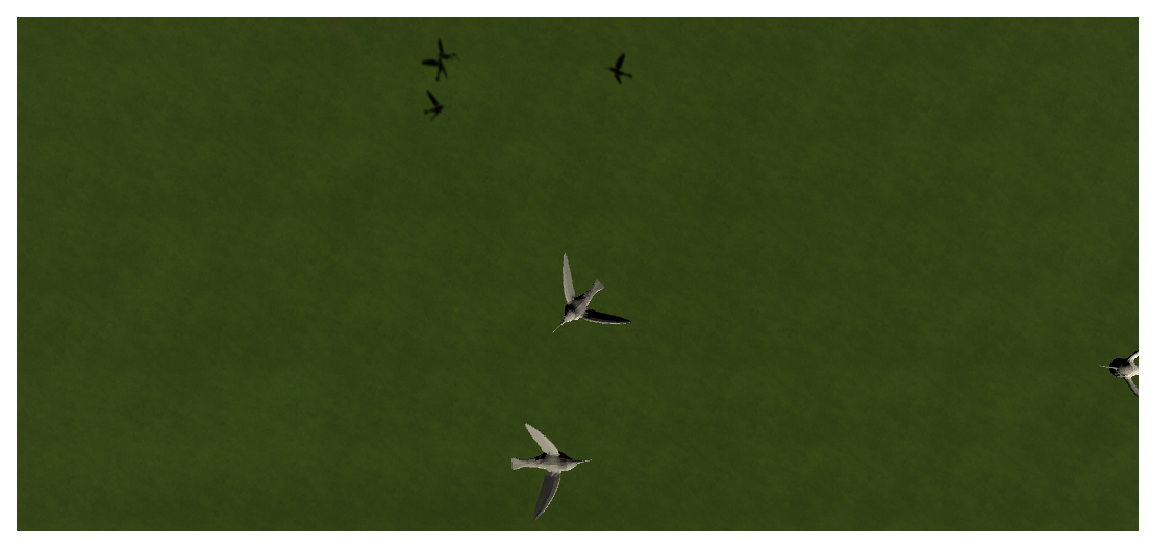
\includegraphics[width=.4\textwidth]{avoid_top.eps}}\hspace{\fill}
\subfloat[Result with $\lambda_{f}=0$ (top view)]{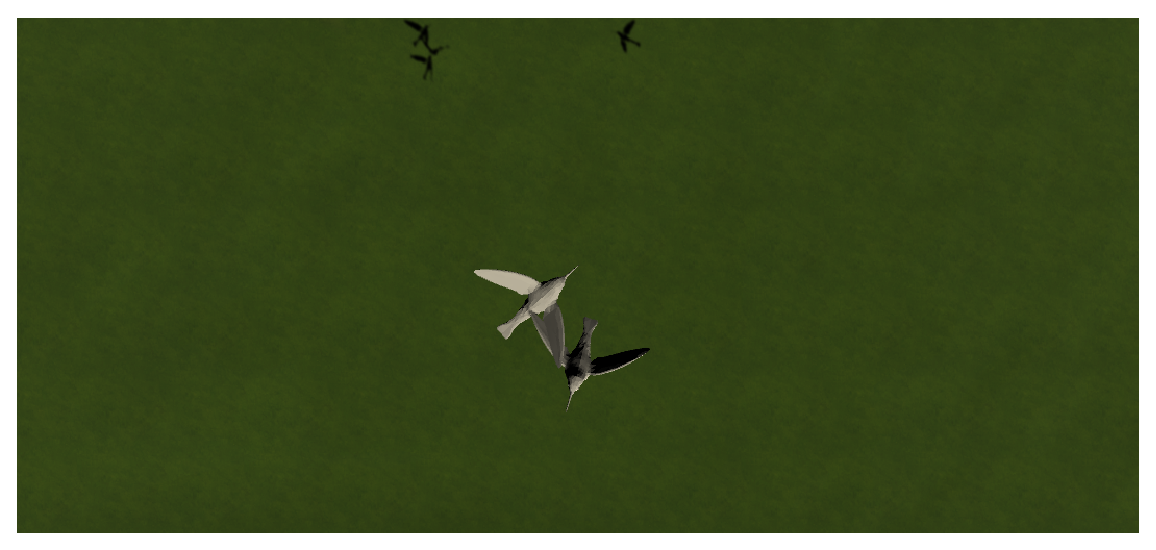
\includegraphics[width=.4\textwidth]{collide_top.eps}}
\end{center}
\caption{Comparison between results with flock behavior similarity term on and off.}
\label{figure:collide}
\end{figure}


However, since result 1 is too short and lack of numbers to observe flock behavior, we use generated video instead for testing with various conditions. Based on our observation on bird flocks, we think that bird flock can be categorized into two types: united flock and separate flock, depending on the relativity between birds in a flock. Thus, we decide to make two kinds of bird flocks to test if the system is capable of having these two kinds of flock motion.


Figure \ref{figure:result2_com1} and Figure \ref{figure:result2_com2} show an result with a video generated by our flock simulation system. The video is relatively long and has 10 birds flying around an object in a united form. Birds fly in similar direction during the whole video. This video is used to evaluate the ability of video with standard united flocks. In the generated flock motion, flock behavior can be observed: birds stay united and collision avoidance is well done. Turning of the flock happens in frame 80 and 100, and the generated motion also turns smoothly, based on trajectory smoothness term in optimization algorithm. This result shows that turning scenario is also handled well even the depth is unknown in the original video.


\begin{figure}[h]
\begin{center}
\subfloat[Input video]{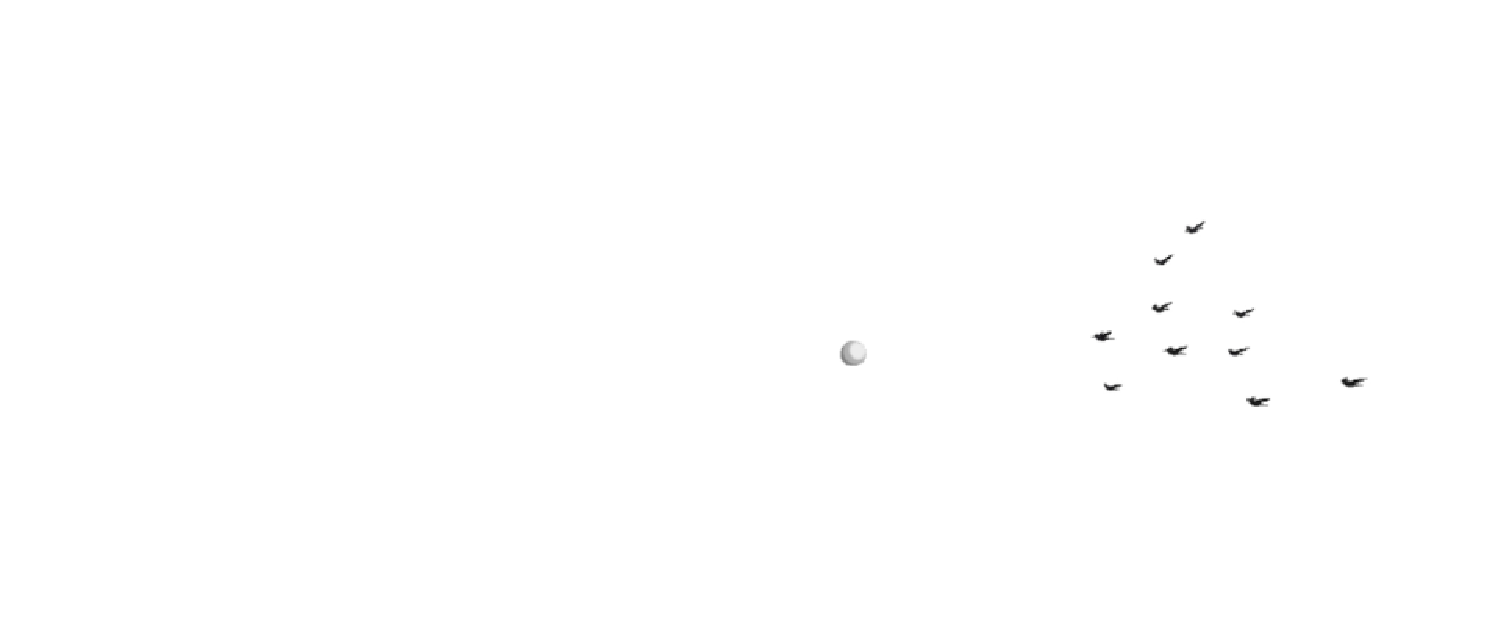
\includegraphics[width=.3\textwidth]{result_2_input_0.eps}}\hspace{\fill}
\subfloat[]{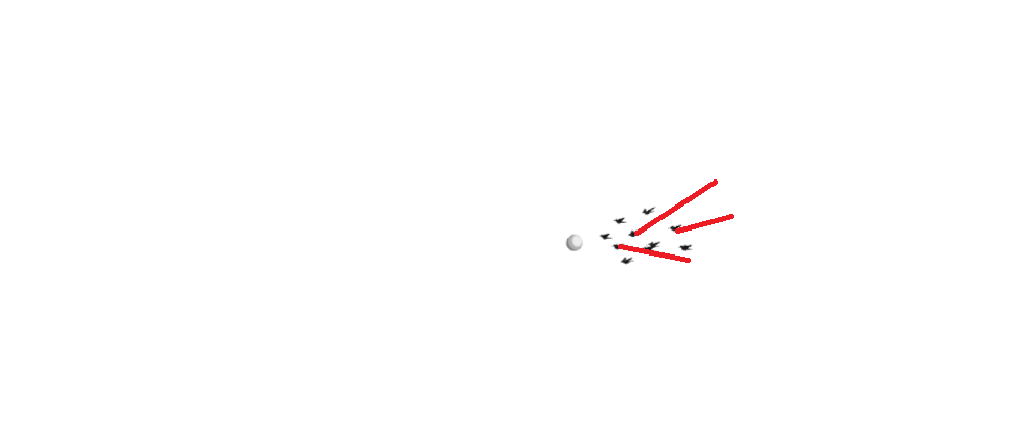
\includegraphics[width=.3\textwidth]{result_2_input_20.eps}}\hspace{\fill}
\subfloat[]{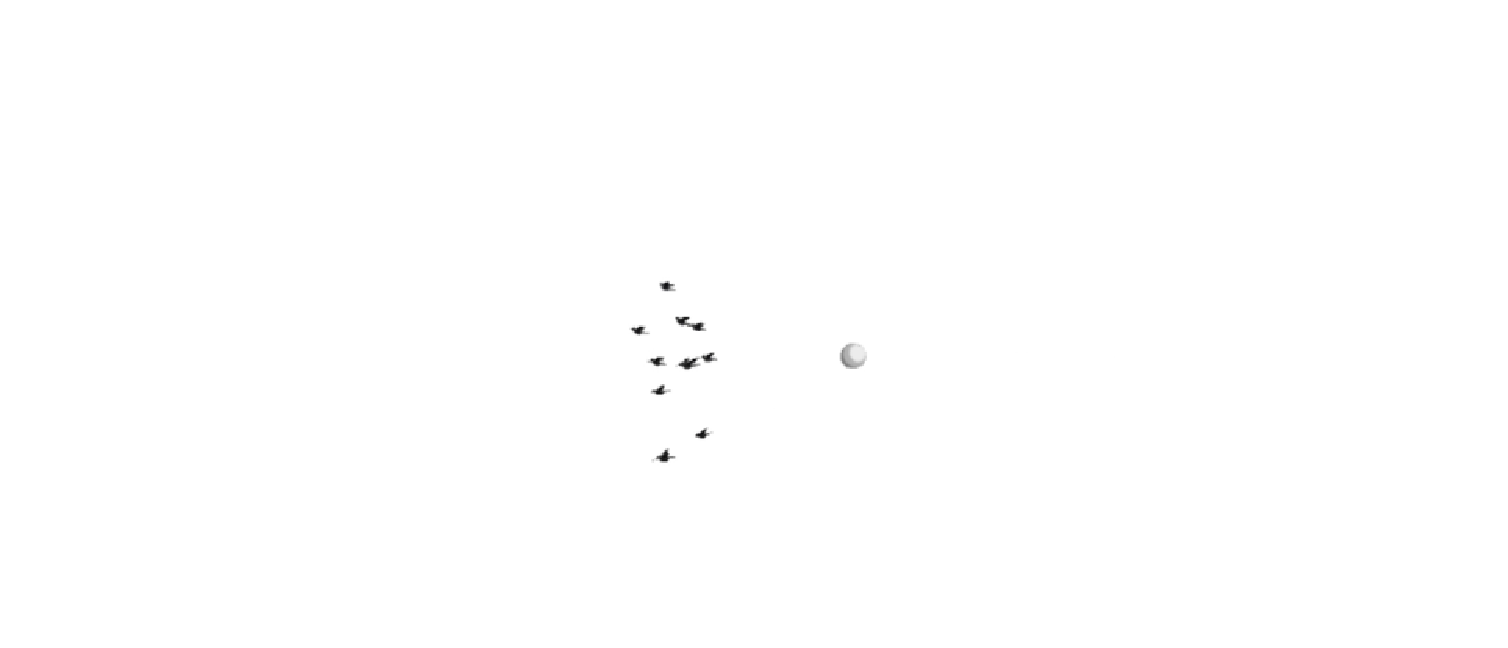
\includegraphics[width=.3\textwidth]{result_2_input_40.eps}}


\subfloat[Result (camera view)]{\includegraphics[width=.3\textwidth]{result_2_side_0.eps}}\hspace{\fill}
\subfloat[]{\includegraphics[width=.3\textwidth]{result_2_side_20.eps}}\hspace{\fill}
\subfloat[]{\includegraphics[width=.3\textwidth]{result_2_side_40.eps}}


\subfloat[Result (top view)]{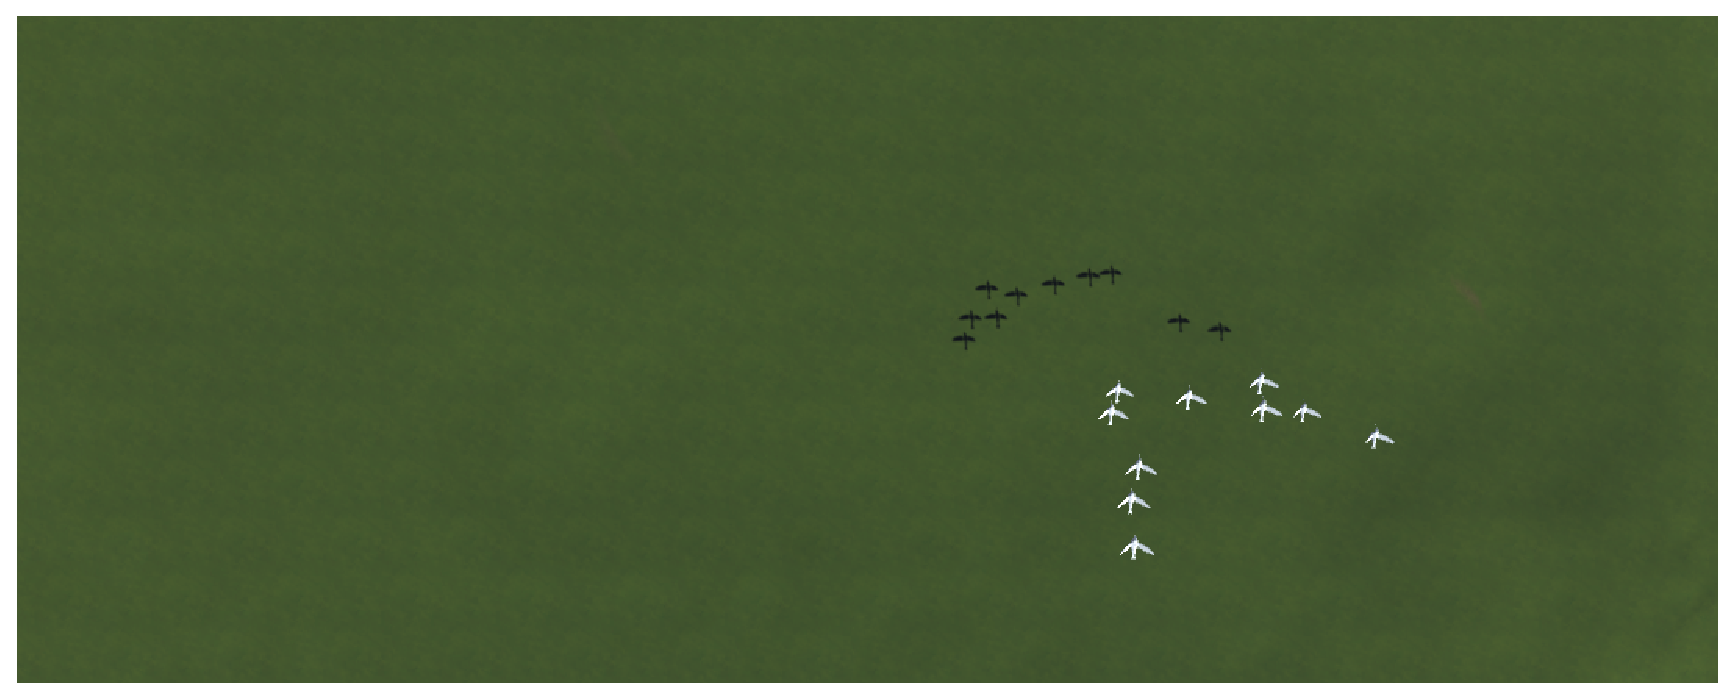
\includegraphics[width=.3\textwidth]{result_2_top_0.eps}}\hspace{\fill}
\subfloat[]{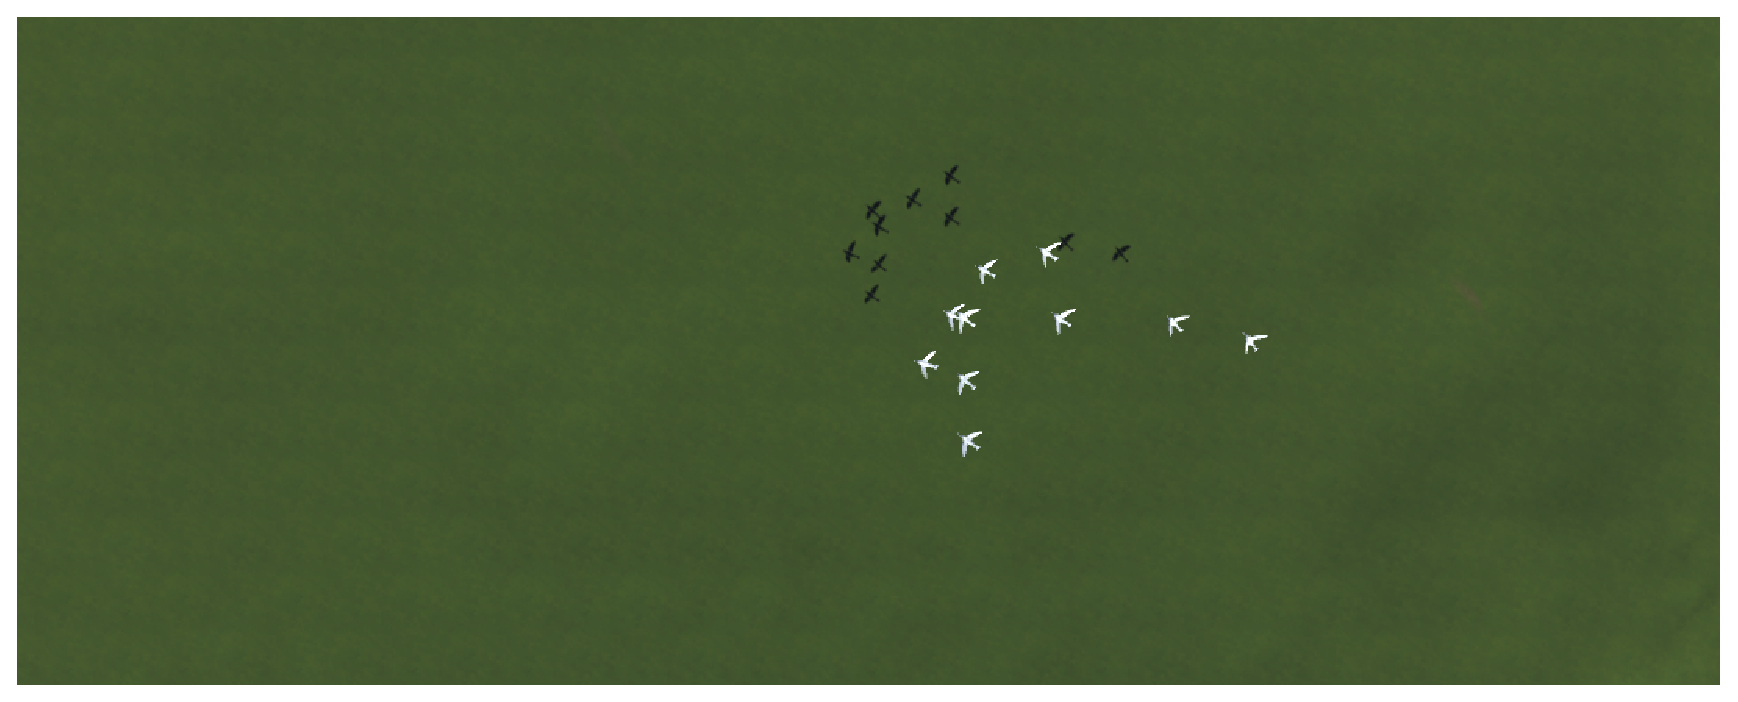
\includegraphics[width=.3\textwidth]{result_2_top_20.eps}}\hspace{\fill}
\subfloat[]{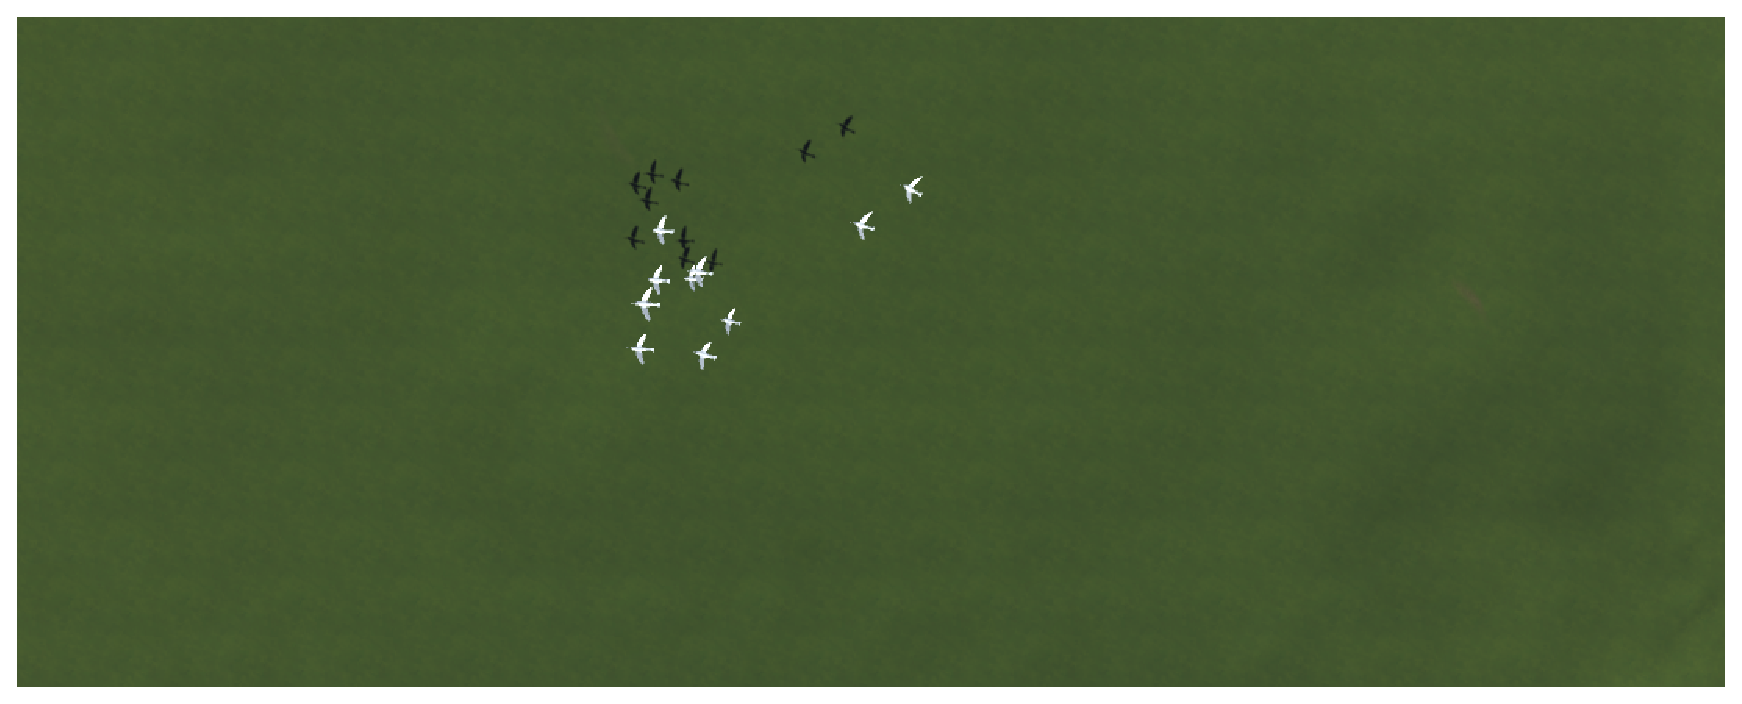
\includegraphics[width=.3\textwidth]{result_2_top_40.eps}}
\end{center}
\caption{Comparison of Result 2 in frame 0, 20, 40.}
\label{figure:result2_com1}
\end{figure}


\begin{figure}[h]
\begin{center}
\subfloat[Input video]{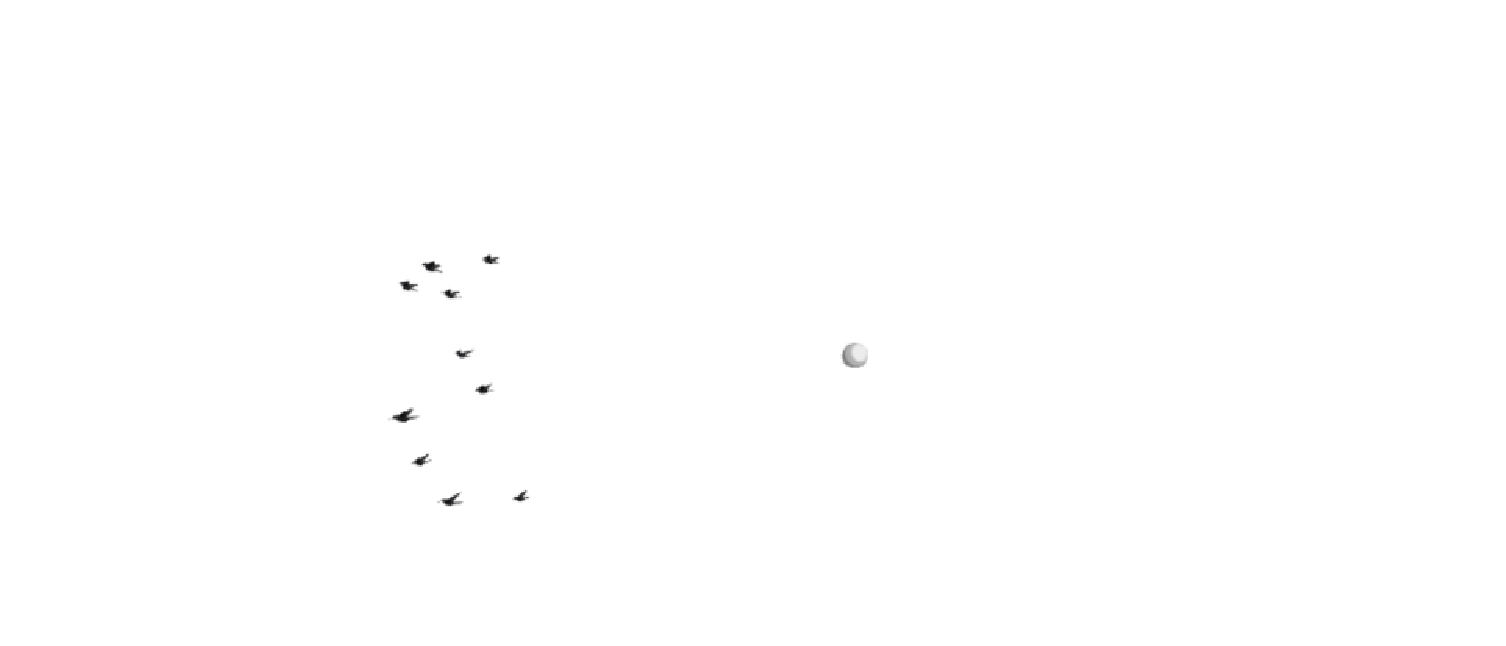
\includegraphics[width=.3\textwidth]{result_2_input_60.eps}}\hspace{\fill}
\subfloat[]{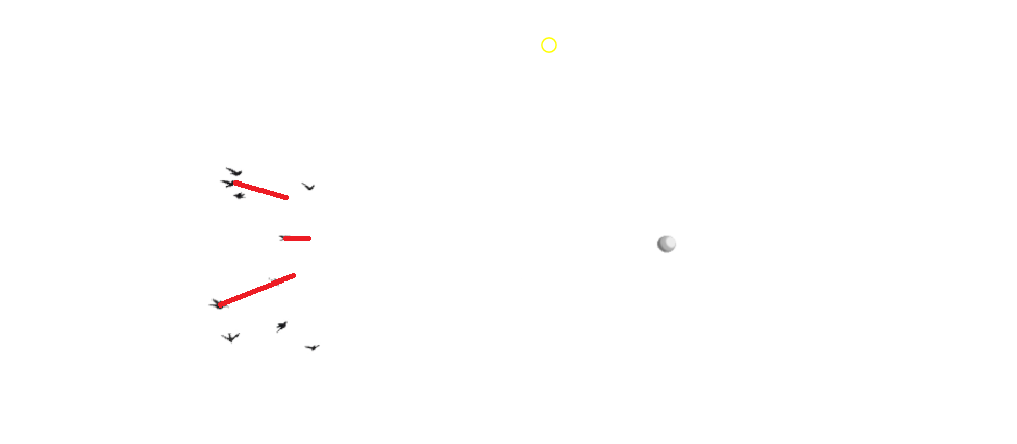
\includegraphics[width=.3\textwidth]{result_2_input_80.eps}}\hspace{\fill}
\subfloat[]{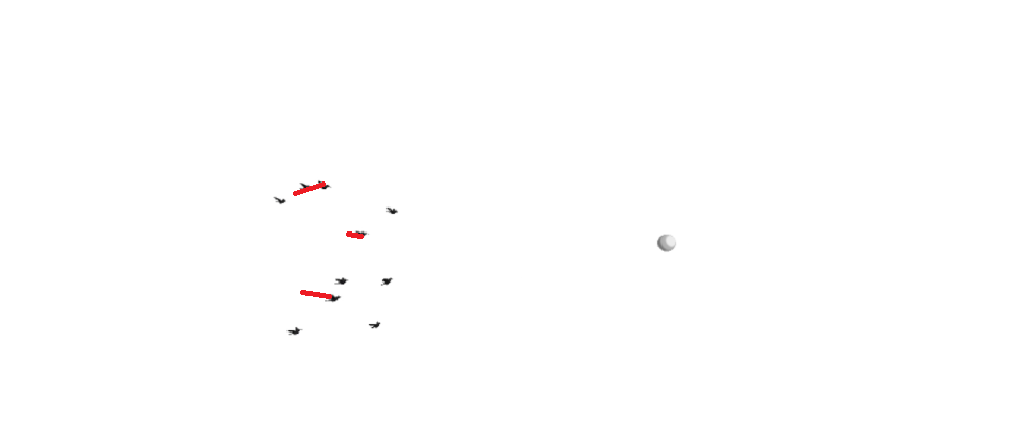
\includegraphics[width=.3\textwidth]{result_2_input_100.eps}}


\subfloat[Result (camera view)]{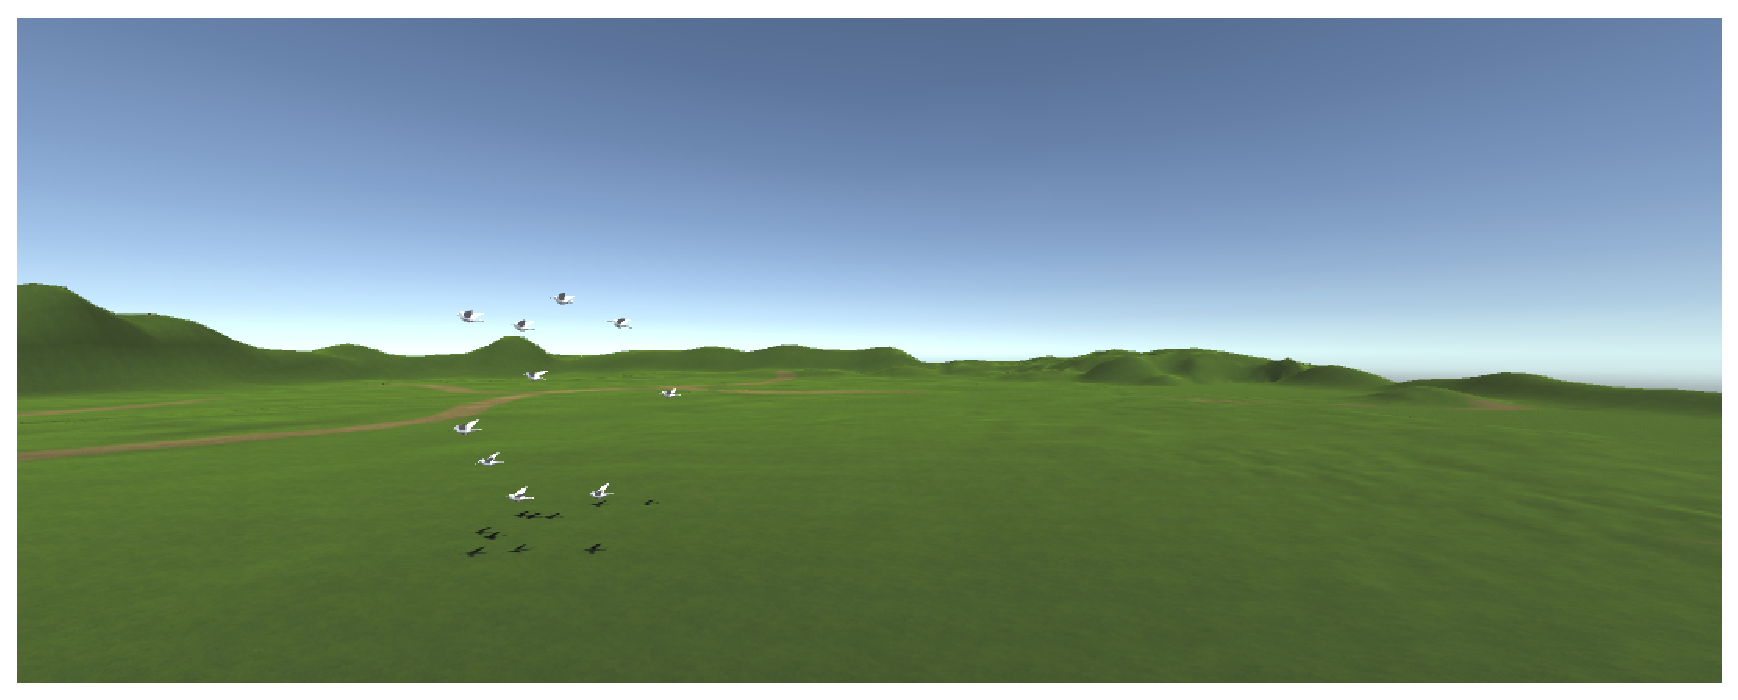
\includegraphics[width=.3\textwidth]{result_2_side_60.eps}}\hspace{\fill}
\subfloat[]{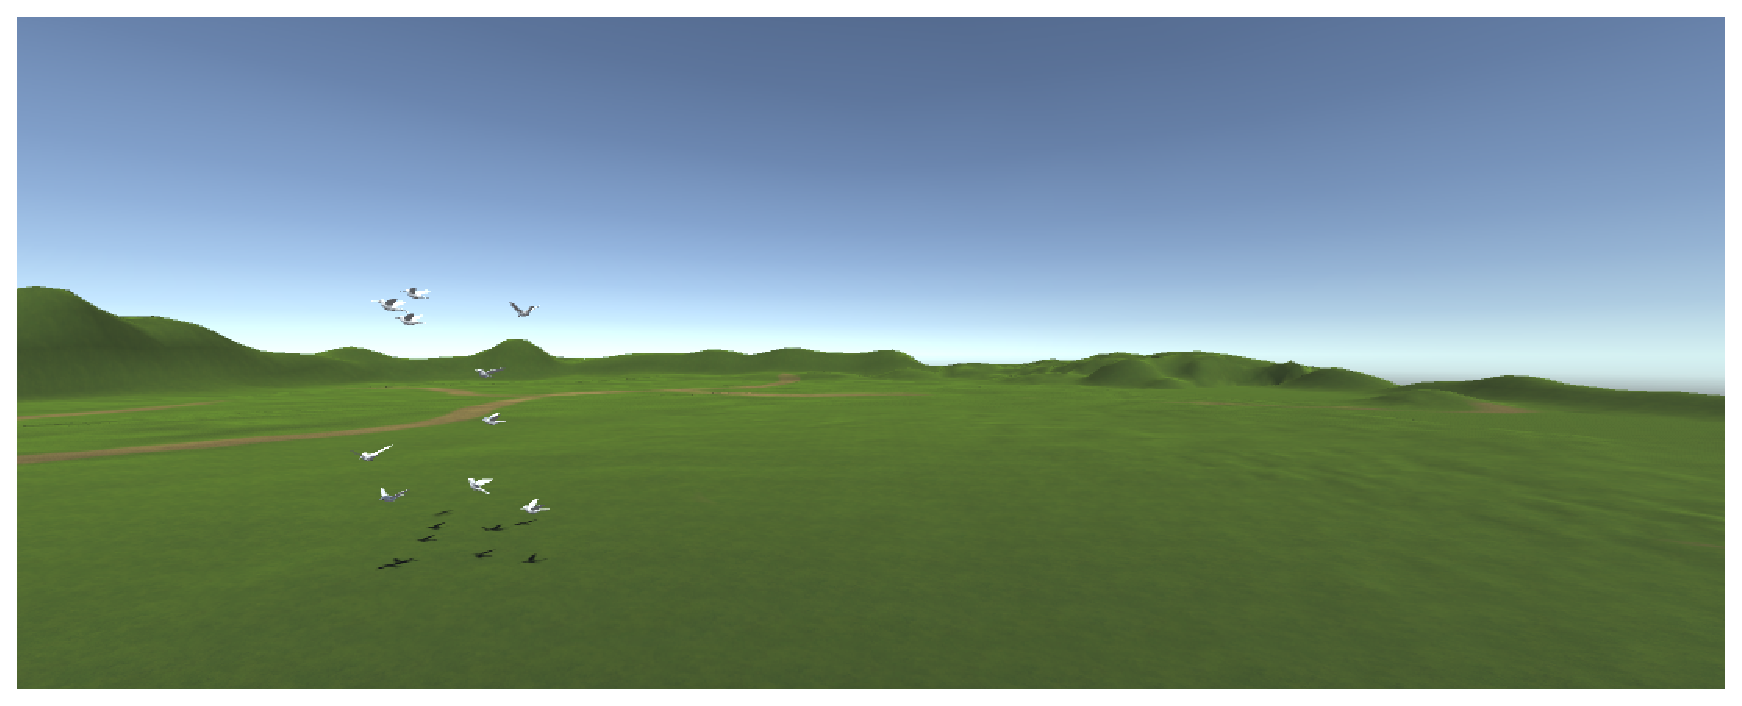
\includegraphics[width=.3\textwidth]{result_2_side_80.eps}}\hspace{\fill}
\subfloat[]{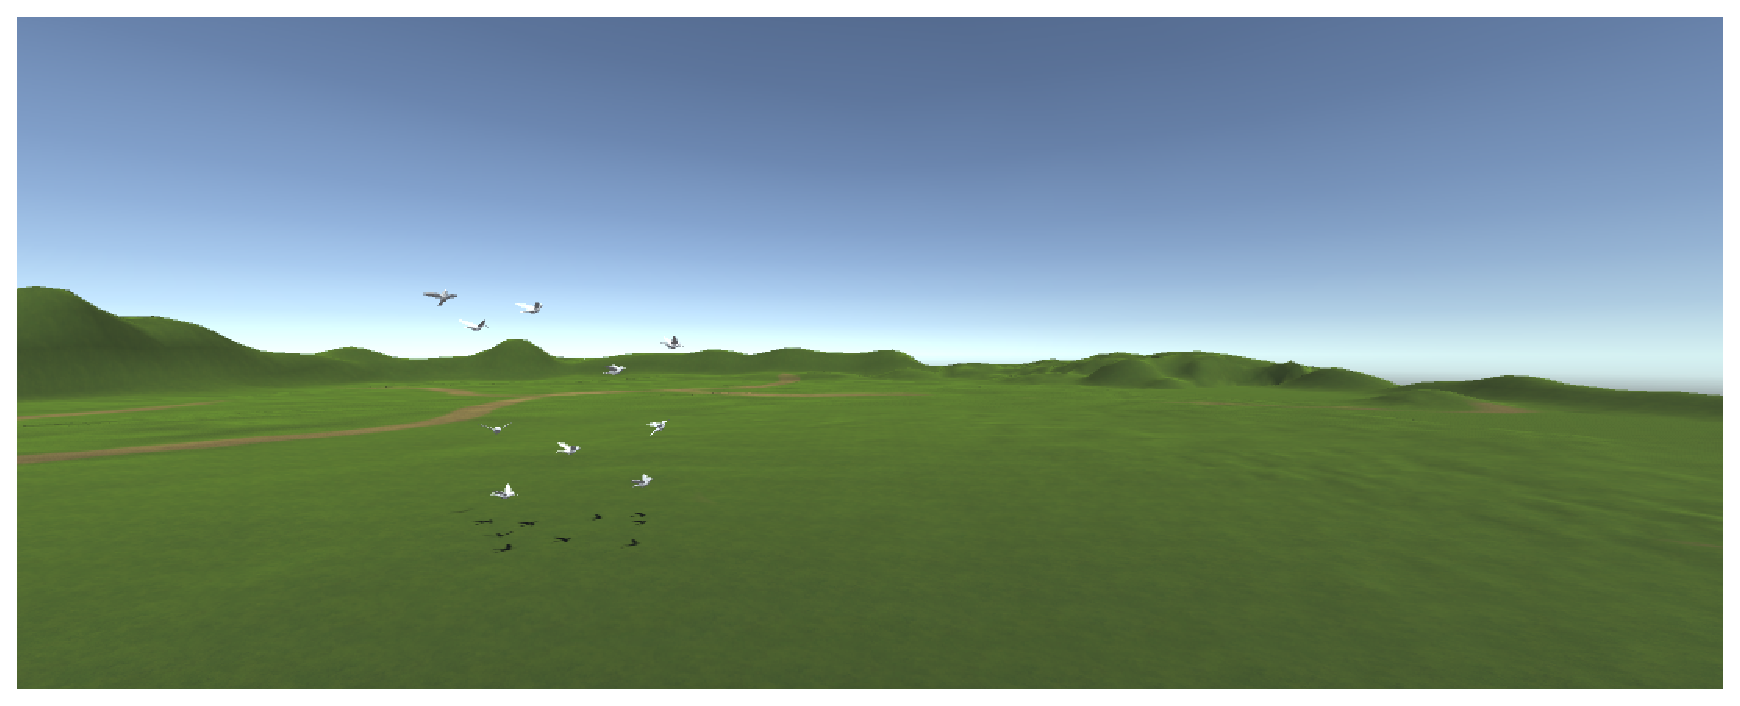
\includegraphics[width=.3\textwidth]{result_2_side_100.eps}}


\subfloat[Result (top view)]{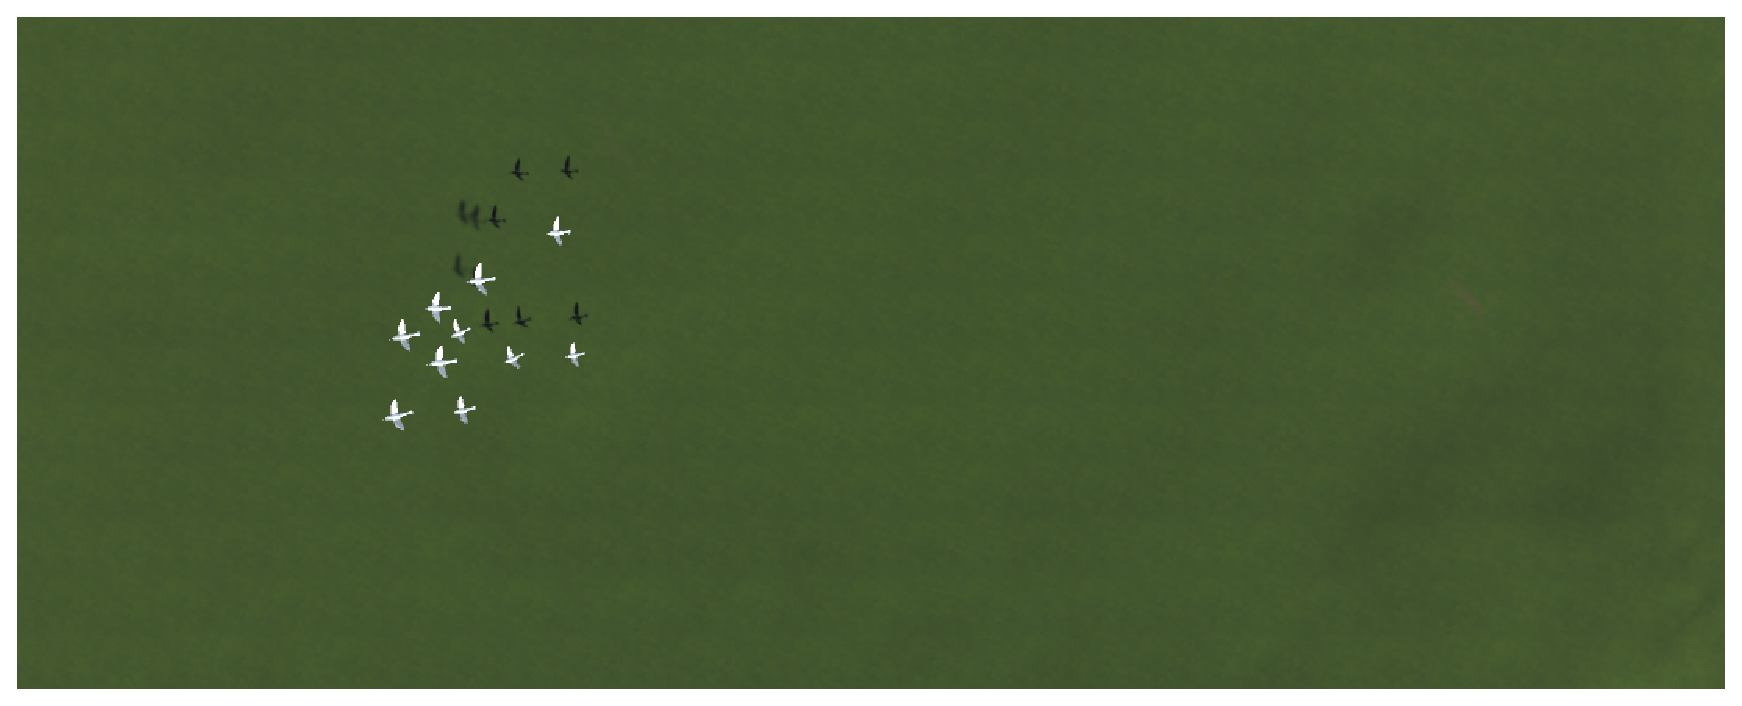
\includegraphics[width=.3\textwidth]{result_2_top_60.eps}}\hspace{\fill}
\subfloat[]{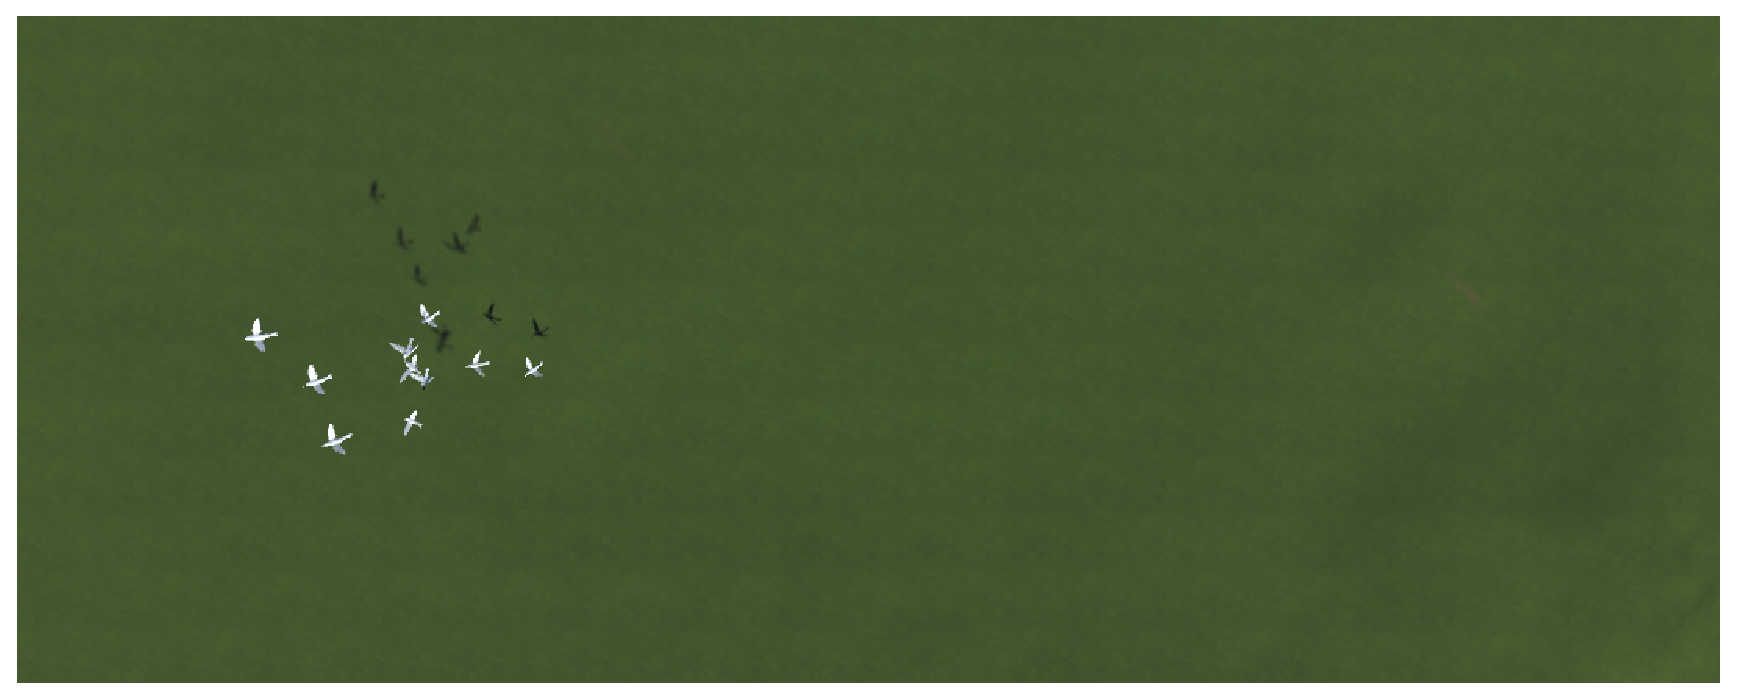
\includegraphics[width=.3\textwidth]{result_2_top_80.eps}}\hspace{\fill}
\subfloat[]{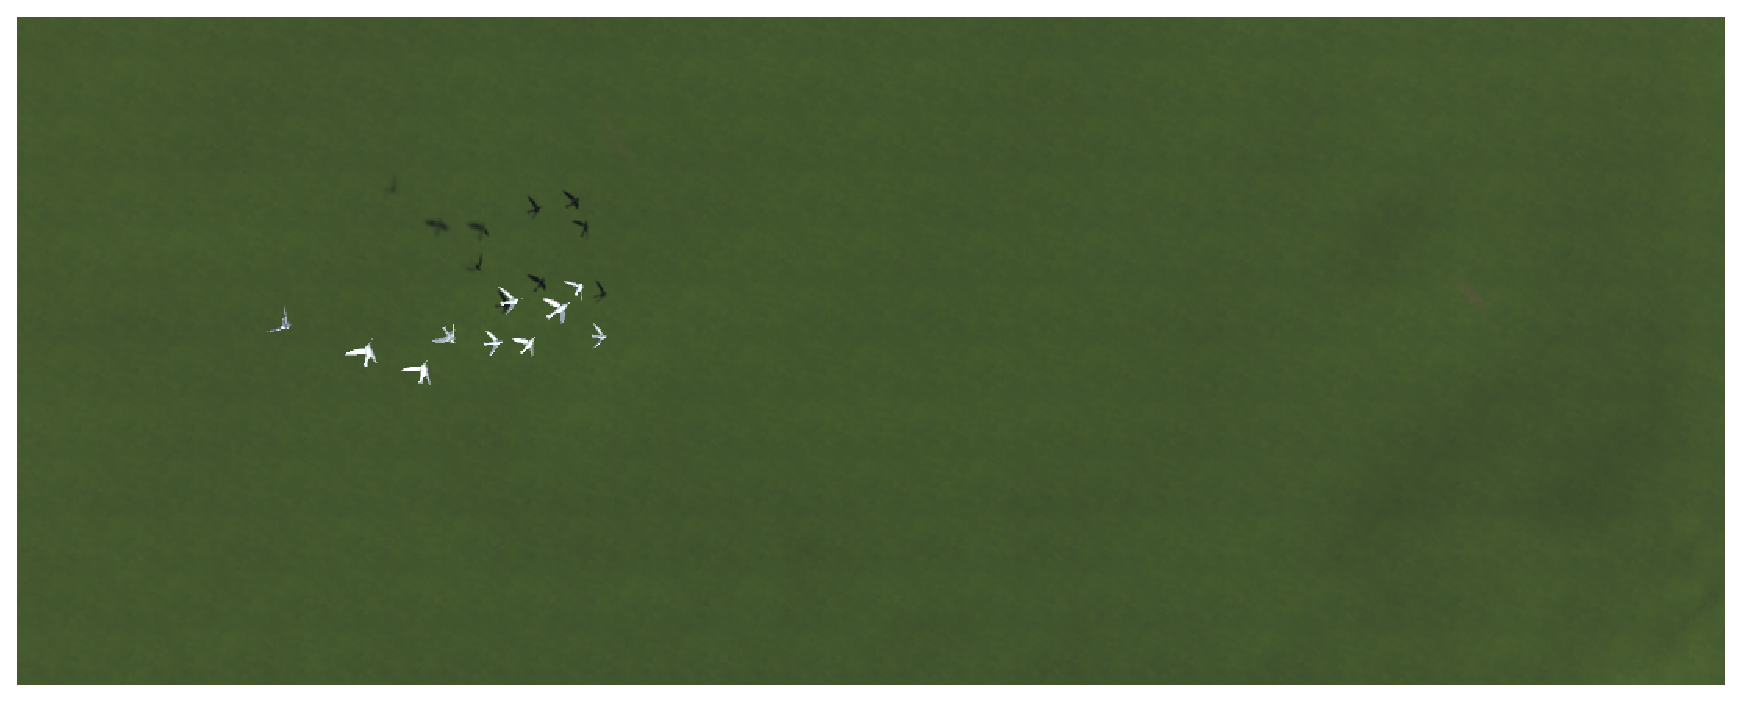
\includegraphics[width=.3\textwidth]{result_2_top_100.eps}}
\end{center}
\caption{Comparison of Result 2 in frame 60, 80, 100.}
\label{figure:result2_com2}
\end{figure}



Figure \ref{figure:result3_com} shows another result with a video generated by simulation. We test our system with this video to observe if birds in the original video fly towards camera. In such scenario, the change in projected position is relative small, meaning that the change in depth is considered to be large. As a result, the generated motion is different with expected: birds leave the camera instead of approaching camera like those in original video. However, this is also and acceptable result, since our goal is not reconstructing the original flock motion. The result still shows a visually plausible in flight trajectory and keeps the birds united. This result shows that our system is also capable of generating flock motion from various kinds of bird flock in the input video.


\begin{figure}[h]
\begin{center}
\subfloat[Input video]{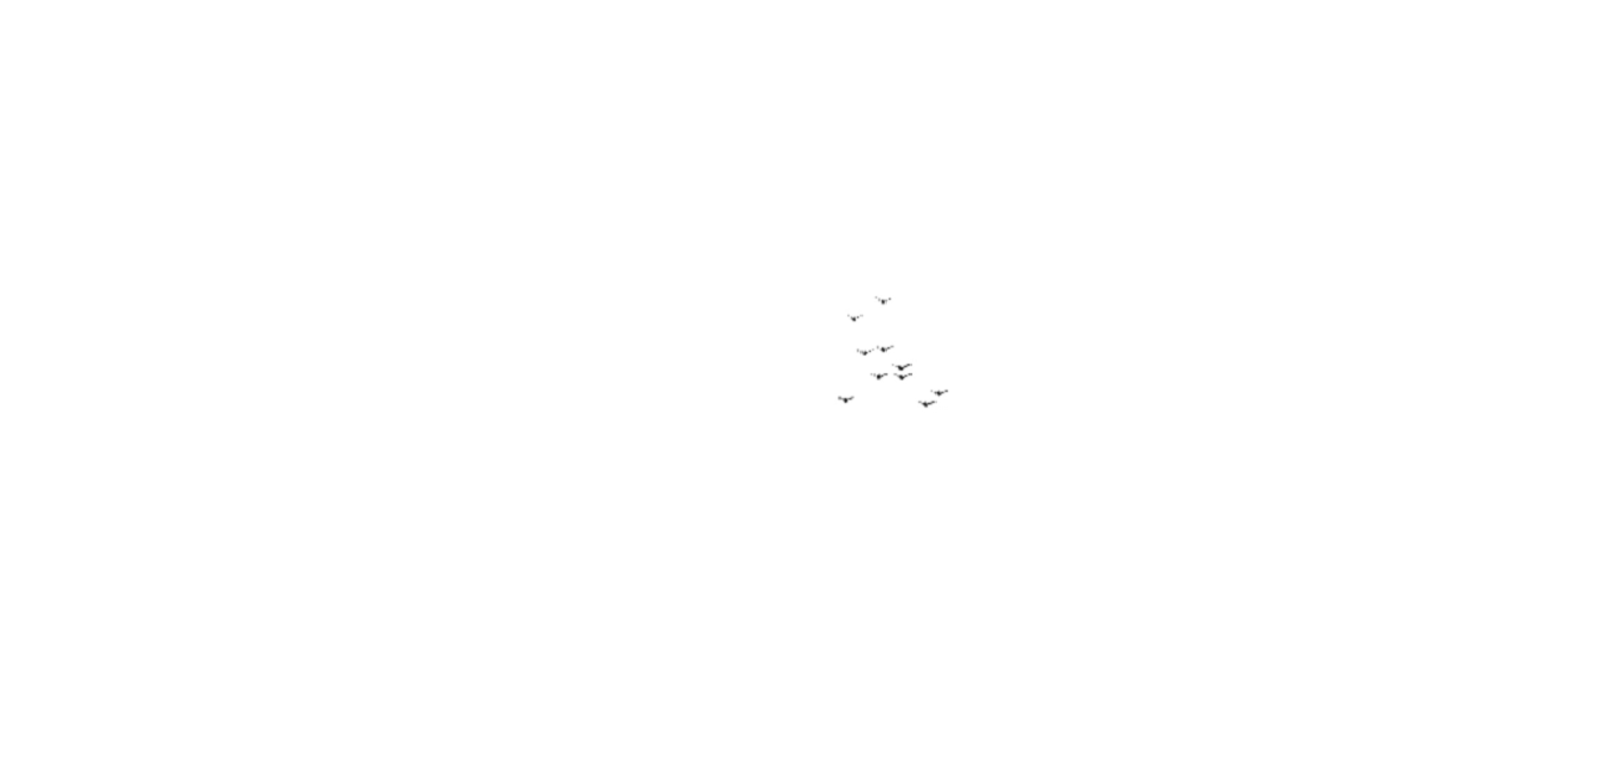
\includegraphics[width=.3\textwidth]{result_3_input_0.eps}}\hspace{\fill}
\subfloat[]{\includegraphics[width=.3\textwidth]{result_3_input_30.eps}}\hspace{\fill}
\subfloat[]{\includegraphics[width=.3\textwidth]{result_3_input_60.eps}}


\subfloat[Result (camera view)]{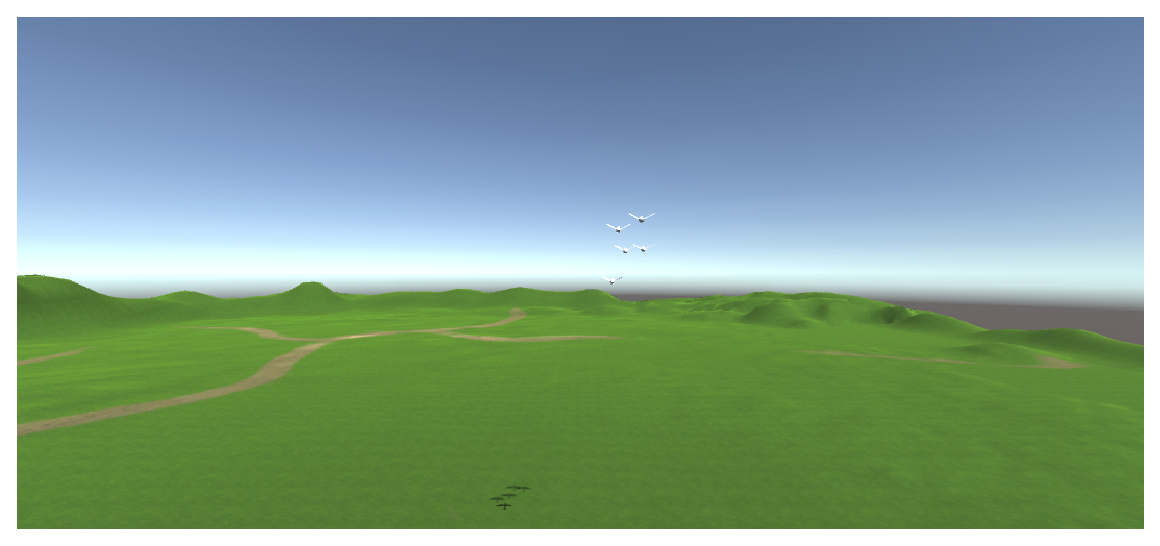
\includegraphics[width=.3\textwidth]{result_3_side_0.eps}}\hspace{\fill}
\subfloat[]{\includegraphics[width=.3\textwidth]{result_3_side_30.eps}}\hspace{\fill}
\subfloat[]{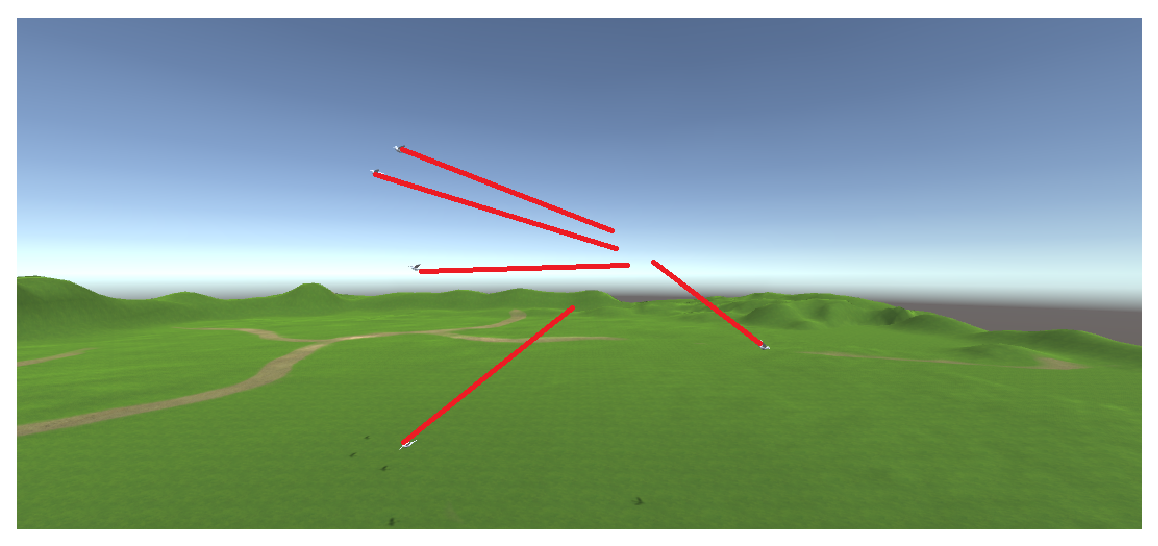
\includegraphics[width=.3\textwidth]{result_3_side_60.eps}}


\subfloat[Result (top view)]{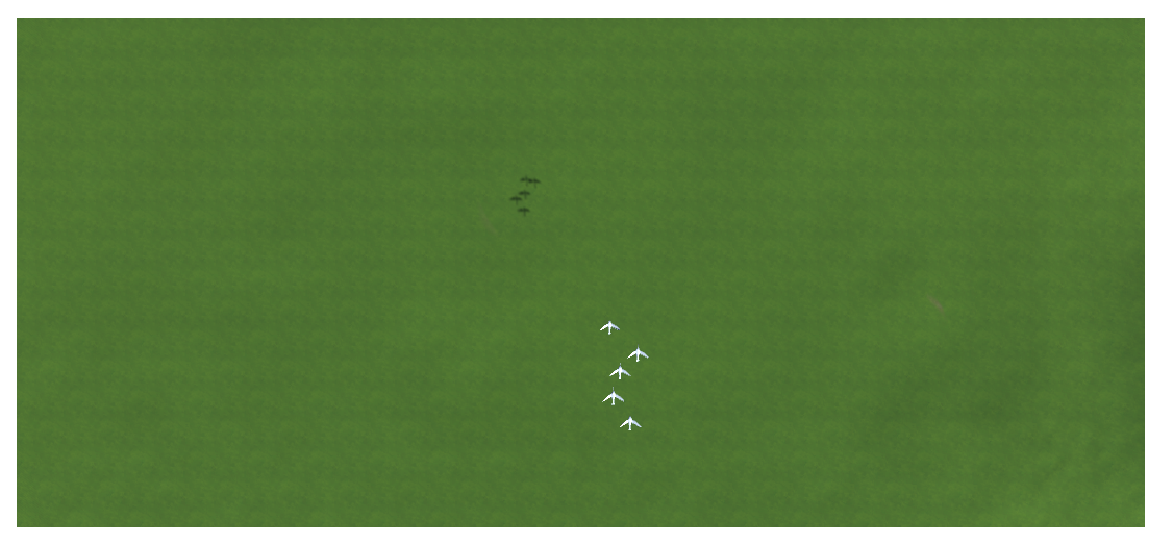
\includegraphics[width=.3\textwidth]{result_3_top_0.eps}}\hspace{\fill}
\subfloat[]{\includegraphics[width=.3\textwidth]{result_3_top_30.eps}}\hspace{\fill}
\subfloat[]{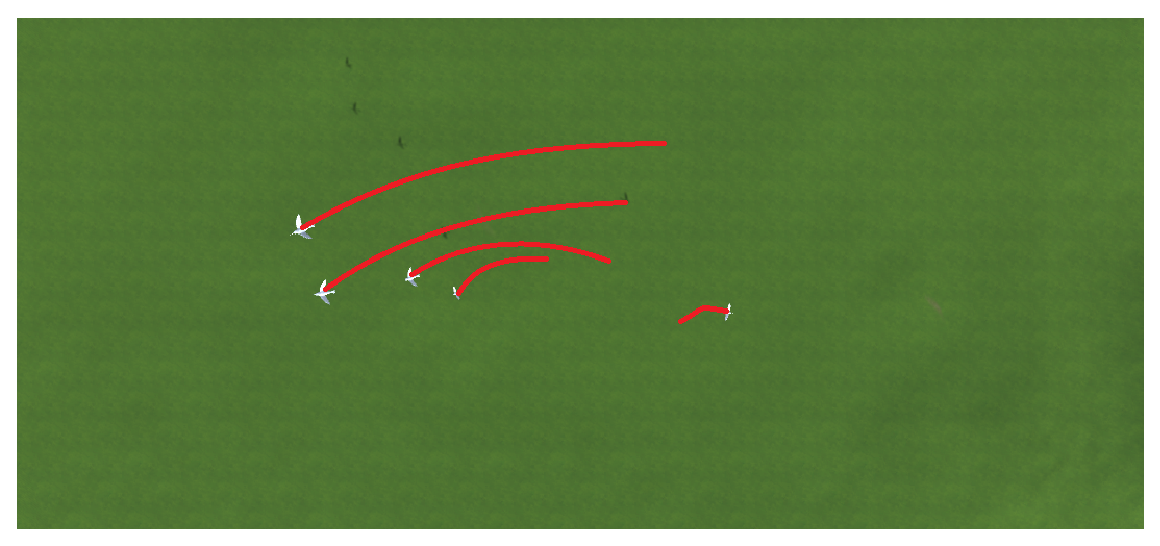
\includegraphics[width=.3\textwidth]{result_3_top_60.eps}}
\end{center}
\caption{Comparison of Result 3 in frame 0, 30, 60.}
\label{figure:result3_com}
\end{figure}